\SourceLeaf{2}
\thispagestyle{empty}
\vspace*{1cm}
\begin{center}
\textsc{CARL FRIEDRICH GAUSS WERKE}

\bigskip

\textsc{BAND I.}
\end{center}
\clearpage

\SourceLeaf{4}
\thispagestyle{empty}
\vspace*{1cm}
\begin{center}
\textsc{CARL FRIEDRICH GAUSS}

\bigskip

{\Large\textsc{WERKE}}

\medskip

\textsc{ERSTER BAND}

\bigskip

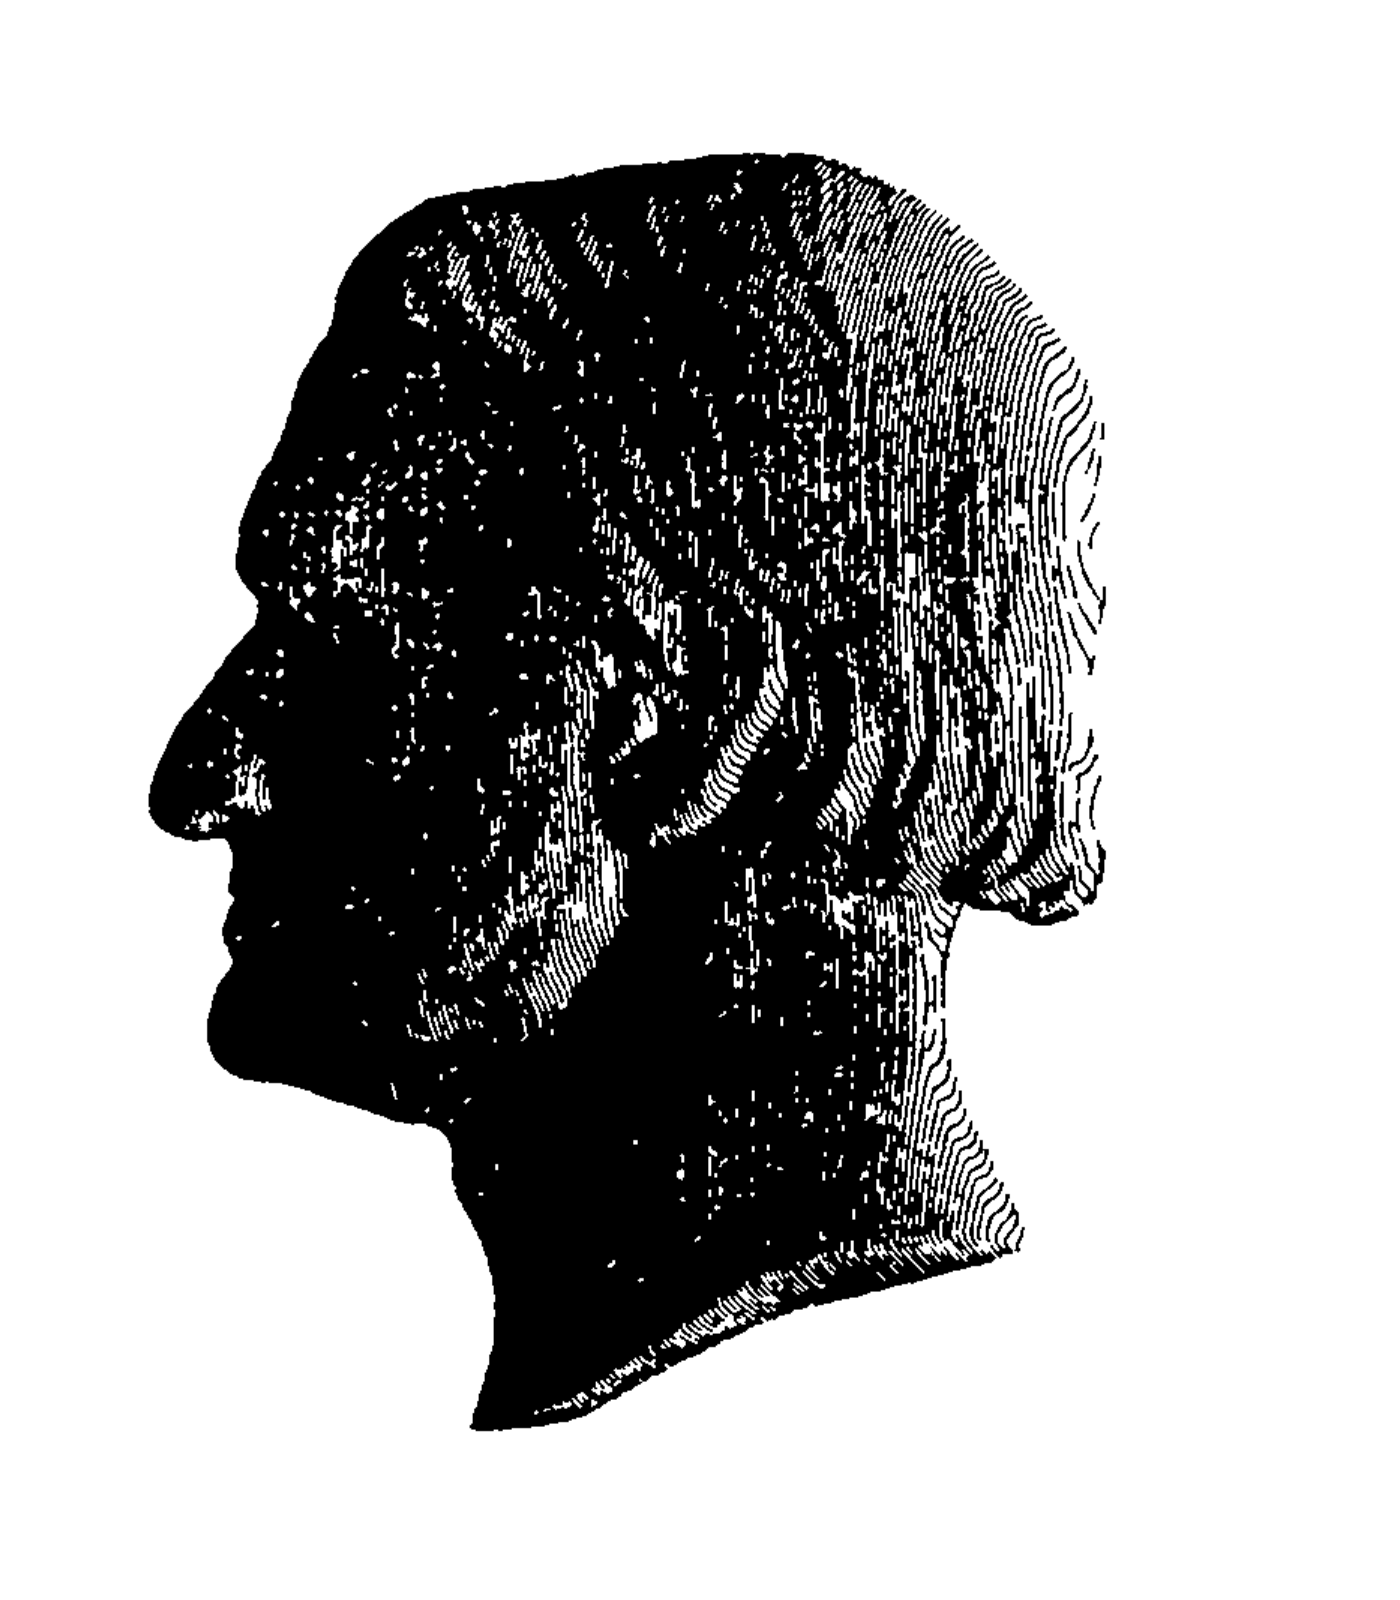
\includegraphics[width=0.30\linewidth]{assets/gauss_portrait.png}

\bigskip

\textsc{HERAUSGEGEBEN}

\smallskip

{\scriptsize VON DER}

\smallskip

\textsc{KÖNIGLICHEN GESELLSCHAFT DER WISSENSCHAFTEN}

{\scriptsize ZU}

\textsc{GÖTTINGEN}

\bigskip

1863.
\end{center}
\clearpage

\SourceLeaf{6}
\thispagestyle{empty}
\vspace*{1cm}
\begin{center}
{\Large\textsc{DISQUISITIONES}}

\medskip

{\Large\textsc{ARITHMETICAE}}

\bigskip

\textsc{AUCTORE}

\bigskip

\textsc{D. CAROLO FRIDERICO GAUSS.}

\bigskip

\BookRule{0.45\linewidth}

\bigskip

\textsc{LIPSIAE}

\medskip

\textsc{IN COMMISSIS APUD GERH. FLEISCHER JUN.}

\bigskip

1801.
\end{center}
\clearpage
